\documentclass[border=4pt]{standalone}
\usepackage{amsmath,amssymb}
\usepackage{tikz}
\usetikzlibrary{arrows.meta,calc}
\newcommand{\bx}[6]{\draw[#5] (#1,#2) rectangle (#3,#4);
  \node[anchor=north west, text width=\dimexpr #3cm-#1cm-0.4cm\relax, align=left, font=\footnotesize, inner sep=0pt] at ({#1+0.2},{#4-0.18}) {#6};}
\tikzset{
 base/.style={rounded corners=3pt, line width=0.5pt},
 learn/.style={base, draw=red!60!black, fill=red!5},
 pol/.style={base, draw=violet!70!black, fill=violet!8},
 net/.style={base, draw=violet!70!black, fill=violet!14},
 netc/.style={base, draw=violet!70!black, dashed, fill=violet!3},
 ifc/.style={base, draw=blue!60!black, fill=blue!7},
 core/.style={base, draw=orange!70!black, dashed, fill=orange!3},
 fast/.style={base, draw=green!45!black, fill=green!10},
 ffw/.style={base, draw=orange!70!black, fill=orange!12},
 grt/.style={base, draw=gray!70!black, fill=gray!8},
 plant/.style={base, draw=black!70, fill=gray!18},
 sig/.style={-{Latex[length=2.2mm]}, line width=0.6pt},
 wup/.style={-{Latex[length=2.2mm]}, line width=0.7pt, dashed, red!60!black},
 lab/.style={font=\scriptsize, inner sep=1.5pt}
}
\begin{document}
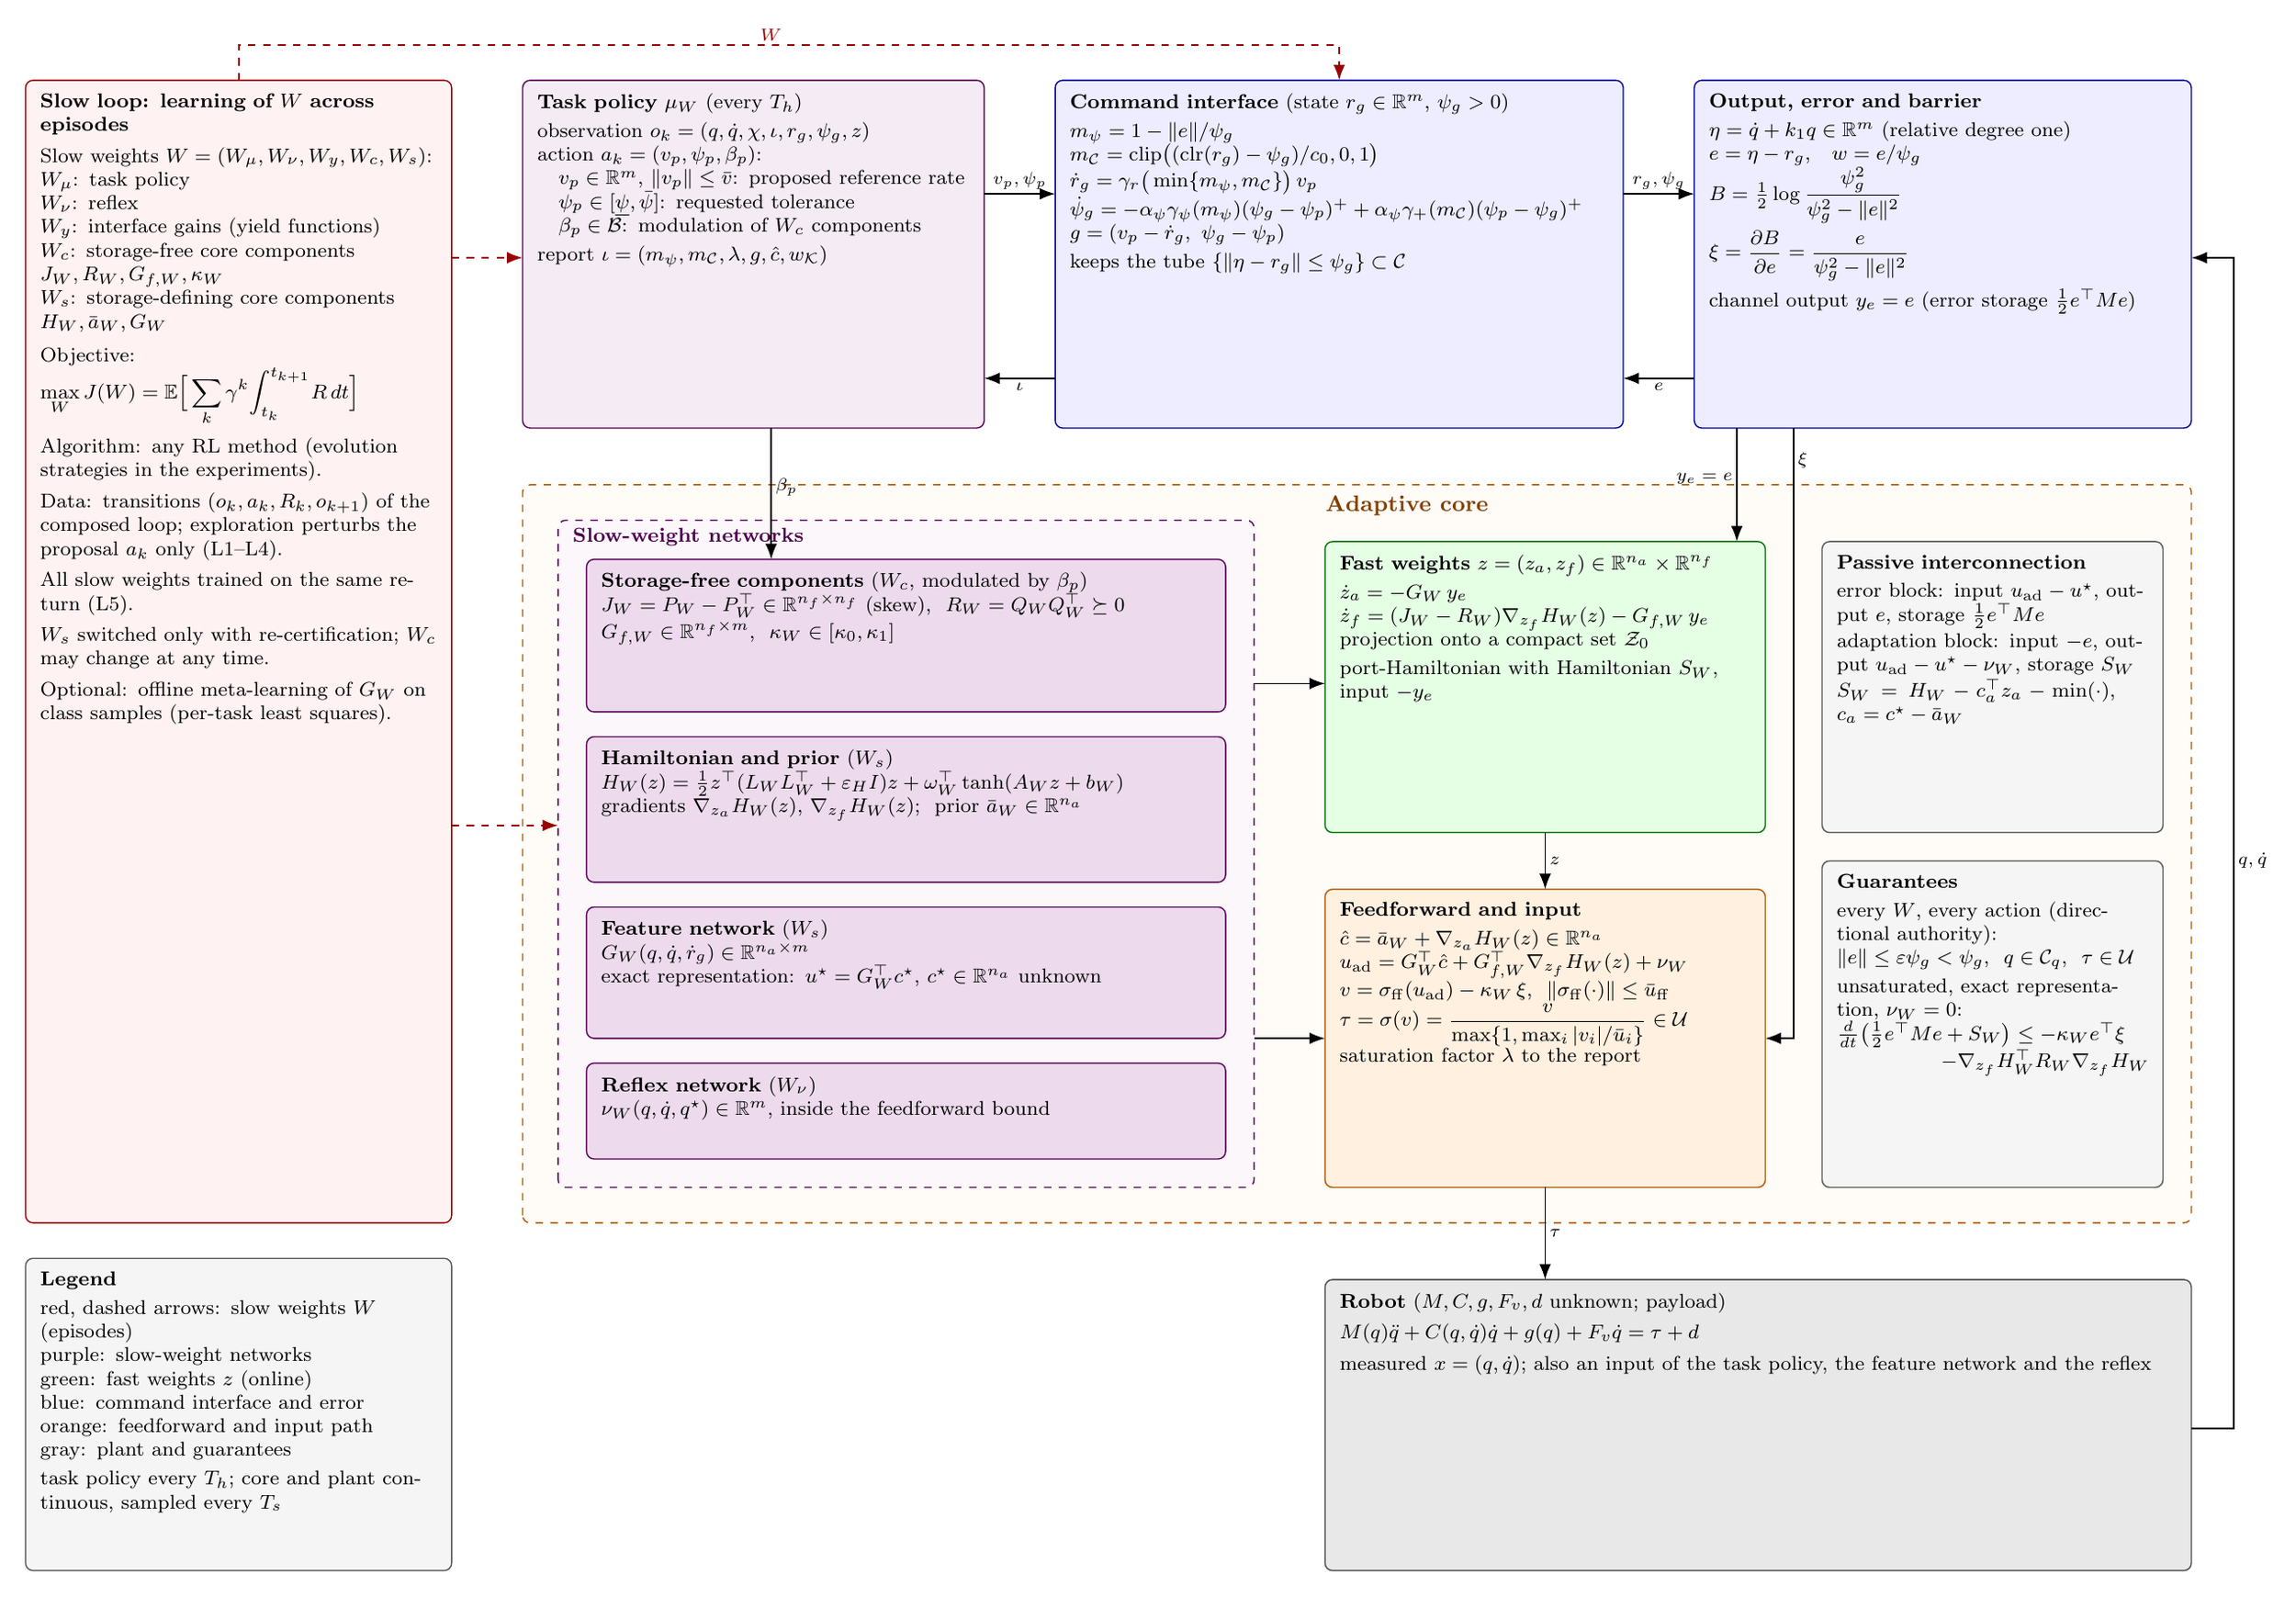
\begin{tikzpicture}[x=1cm,y=1cm]
\bx{0.5}{5.4}{6.5}{21.5}{learn}{\textbf{Slow loop: learning of $W$ across episodes}\\[3pt]
Slow weights $W=(W_\mu,W_\nu,W_y,W_c,W_s)$:\\
$W_\mu$: task policy\\
$W_\nu$: reflex\\
$W_y$: interface gains (yield functions)\\
$W_c$: storage-free core components $J_W,R_W,G_{f,W},\kappa_W$\\
$W_s$: storage-defining core components $H_W,\bar a_W,G_W$\\[4pt]
Objective:\\
$\displaystyle\max_W J(W)=\mathbb E\Big[\sum_k\gamma^k\!\int_{t_k}^{t_{k+1}}\!R\,dt\Big]$\\[4pt]
Algorithm: any RL method (evolution strategies in the experiments).\\[3pt]
Data: transitions $(o_k,a_k,R_k,o_{k+1})$ of the composed loop; exploration perturbs the proposal $a_k$ only (L1--L4).\\[3pt]
All slow weights trained on the same return (L5).\\[3pt]
$W_s$ switched only with re-certification; $W_c$ may change at any time.\\[3pt]
Optional: offline meta-learning of $G_W$ on class samples (per-task least squares).}
\bx{0.5}{0.5}{6.5}{4.9}{grt}{\textbf{Legend}\\[2pt]
red, dashed arrows: slow weights $W$ (episodes)\\
purple: slow-weight networks\\
green: fast weights $z$ (online)\\
blue: command interface and error\\
orange: feedforward and input path\\
gray: plant and guarantees\\[2pt]
task policy every $T_h$; core and plant continuous, sampled every $T_s$}
\bx{7.5}{16.6}{14.0}{21.5}{pol}{\textbf{Task policy $\mu_W$} (every $T_h$)\\[2pt]
observation $o_k=(q,\dot q,\chi,\iota,r_g,\psi_g,z)$\\
action $a_k=(v_p,\psi_p,\beta_p)$:\\
\quad $v_p\in\mathbb R^m$, $\|v_p\|\le\bar v$: proposed reference rate\\
\quad $\psi_p\in[\underline\psi,\bar\psi]$: requested tolerance\\
\quad $\beta_p\in\mathcal B$: modulation of $W_c$ components\\[2pt]
report $\iota=(m_\psi,m_{\mathcal C},\lambda,g,\hat c,w_{\mathcal K})$}
\bx{15.0}{16.6}{23.0}{21.5}{ifc}{\textbf{Command interface} (state $r_g\in\mathbb R^m$, $\psi_g>0$)\\[2pt]
$m_\psi=1-\|e\|/\psi_g$\\
$m_{\mathcal C}=\mathrm{clip}\big((\mathrm{clr}(r_g)-\psi_g)/c_0,0,1\big)$\\
$\dot r_g=\gamma_r\big(\min\{m_\psi,m_{\mathcal C}\}\big)\,v_p$\\
$\dot\psi_g=-\alpha_\psi\gamma_\psi(m_\psi)(\psi_g-\psi_p)^+ +\alpha_\psi\gamma_+(m_{\mathcal C})(\psi_p-\psi_g)^+$\\
$g=(v_p-\dot r_g,\ \psi_g-\psi_p)$\\[2pt]
keeps the tube $\{\|\eta-r_g\|\le\psi_g\}\subset\mathcal C$}
\bx{24.0}{16.6}{31.0}{21.5}{ifc}{\textbf{Output, error and barrier}\\[2pt]
$\eta=\dot q+k_1q\in\mathbb R^m$ (relative degree one)\\
$e=\eta-r_g$,\quad $w=e/\psi_g$\\
$B=\tfrac12\log\dfrac{\psi_g^2}{\psi_g^2-\|e\|^2}$\\[2pt]
$\xi=\dfrac{\partial B}{\partial e}=\dfrac{e}{\psi_g^2-\|e\|^2}$\\[2pt]
channel output $y_e=e$ (error storage $\tfrac12e^\top Me$)}
\bx{7.5}{5.4}{31.0}{15.8}{core}{}
\node[anchor=north west, font=\small\bfseries, inner sep=0pt, orange!50!black] at (18.8,15.65) {Adaptive core};
\bx{8.0}{5.9}{17.8}{15.3}{netc}{}
\node[anchor=north west, font=\footnotesize\bfseries, inner sep=0pt, violet!60!black] at (8.2,15.2) {Slow-weight networks};
\bx{8.4}{12.6}{17.4}{14.75}{net}{\textbf{Storage-free components} ($W_c$, modulated by $\beta_p$)\\
$J_W=P_W-P_W^\top\in\mathbb R^{n_f\times n_f}$ (skew), \ $R_W=Q_WQ_W^\top\succeq0$\\
$G_{f,W}\in\mathbb R^{n_f\times m}$, \ $\kappa_W\in[\kappa_0,\kappa_1]$}
\bx{8.4}{10.2}{17.4}{12.25}{net}{\textbf{Hamiltonian and prior} ($W_s$)\\
$H_W(z)=\tfrac12z^\top(L_WL_W^\top+\varepsilon_HI)z+\omega_W^\top\tanh(A_Wz+b_W)$\\
gradients $\nabla_{z_a}H_W(z)$, $\nabla_{z_f}H_W(z)$; \ prior $\bar a_W\in\mathbb R^{n_a}$}
\bx{8.4}{8.0}{17.4}{9.85}{net}{\textbf{Feature network} ($W_s$)\\
$G_W(q,\dot q,\dot r_g)\in\mathbb R^{n_a\times m}$\\
exact representation: $u^\star=G_W^\top c^\star$, $c^\star\in\mathbb R^{n_a}$ unknown}
\bx{8.4}{6.3}{17.4}{7.65}{net}{\textbf{Reflex network} ($W_\nu$)\\
$\nu_W(q,\dot q,q^\star)\in\mathbb R^m$, inside the feedforward bound}
\bx{18.8}{10.9}{25.0}{15.0}{fast}{\textbf{Fast weights} $z=(z_a,z_f)\in\mathbb R^{n_a}\times\mathbb R^{n_f}$\\[2pt]
$\dot z_a=-G_W\,y_e$\\
$\dot z_f=(J_W-R_W)\nabla_{z_f}H_W(z)-G_{f,W}\,y_e$\\
projection onto a compact set $\mathcal Z_0$\\[2pt]
port-Hamiltonian with Hamiltonian $S_W$, input $-y_e$}
\bx{18.8}{5.9}{25.0}{10.1}{ffw}{\textbf{Feedforward and input}\\[2pt]
$\hat c=\bar a_W+\nabla_{z_a}H_W(z)\in\mathbb R^{n_a}$\\
$u_{\mathrm{ad}}=G_W^\top\hat c+G_{f,W}^\top\nabla_{z_f}H_W(z)+\nu_W$\\
$v=\sigma_{\mathrm{ff}}(u_{\mathrm{ad}})-\kappa_W\,\xi$, \ $\|\sigma_{\mathrm{ff}}(\cdot)\|\le\bar u_{\mathrm{ff}}$\\
$\tau=\sigma(v)=\dfrac{v}{\max\{1,\max_i|v_i|/\bar u_i\}}\in\mathcal U$\\
saturation factor $\lambda$ to the report}
\bx{25.8}{10.9}{30.6}{15.0}{grt}{\textbf{Passive interconnection}\\[2pt]
error block: input $u_{\mathrm{ad}}-u^\star$, output $e$, storage $\tfrac12e^\top Me$\\[1pt]
adaptation block: input $-e$, output $u_{\mathrm{ad}}-u^\star-\nu_W$, storage $S_W$\\[1pt]
$S_W=H_W-c_a^\top z_a-\min(\cdot)$, $c_a=c^\star-\bar a_W$}
\bx{25.8}{5.9}{30.6}{10.5}{grt}{\textbf{Guarantees}\\[2pt]
every $W$, every action (directional authority):\\
$\|e\|\le\varepsilon\psi_g<\psi_g$, \ $q\in\mathcal C_q$, \ $\tau\in\mathcal U$\\[2pt]
unsaturated, exact representation, $\nu_W=0$:\\
$\tfrac{d}{dt}\big(\tfrac12e^\top Me+S_W\big)\le-\kappa_We^\top\xi$\\
\hfill$-\nabla_{z_f}H_W^\top R_W\nabla_{z_f}H_W$}
\bx{18.8}{0.5}{31.0}{4.6}{plant}{\textbf{Robot} ($M,C,g,F_v,d$ unknown; payload)\\[3pt]
$M(q)\ddot q+C(q,\dot q)\dot q+g(q)+F_v\dot q=\tau+d$\\[3pt]
measured $x=(q,\dot q)$; also an input of the task policy, the feature network and the reflex}
\draw[wup] (6.5,19.0) -- (7.5,19.0);
\draw[wup] (6.5,11.0) -- (8.0,11.0);
\draw[wup] (3.5,21.5) -- (3.5,22.0) -- (19.0,22.0) -- (19.0,21.5);
\node[lab, red!60!black, above] at (11.0,22.0) {$W$};
\draw[sig] (14.0,19.9) -- (15.0,19.9) node[lab, midway, above] {$v_p,\psi_p$};
\draw[sig] (15.0,17.3) -- (14.0,17.3) node[lab, midway, below] {$\iota$};
\draw[sig] (11.0,16.6) -- (11.0,14.75) node[lab, pos=0.45, right] {$\beta_p$};
\draw[sig] (23.0,19.9) -- (24.0,19.9) node[lab, midway, above] {$r_g,\psi_g$};
\draw[sig] (24.0,17.3) -- (23.0,17.3) node[lab, midway, below] {$e$};
\draw[sig] (24.6,16.6) -- (24.6,15.0) node[lab, pos=0.45, left] {$y_e=e$};
\draw[sig] (25.4,16.6) -- (25.4,8.0) -- (25.0,8.0);
\node[lab, right] at (25.4,16.15) {$\xi$};
\draw[sig] (17.8,13.0) -- (18.8,13.0);
\draw[sig] (17.8,8.0) -- (18.8,8.0);
\draw[sig] (21.9,10.9) -- (21.9,10.1) node[lab, midway, right] {$z$};
\draw[sig] (21.9,5.9) -- (21.9,4.6) node[lab, midway, right] {$\tau$};
\draw[sig] (31.0,2.5) -- (31.6,2.5) -- (31.6,19.0) -- (31.0,19.0);
\node[lab, right] at (31.6,10.5) {$q,\dot q$};
\end{tikzpicture}
\end{document}
